\documentclass[11pt,a4paper]{article}
\usepackage[utf8]{inputenc}
\usepackage[T1]{fontenc}
\usepackage[english]{babel}
\usepackage{amsmath}
\usepackage{amsfonts}
\usepackage{amssymb}
\usepackage{graphicx}
\usepackage{listings}
\usepackage{xcolor}
\usepackage{hyperref}

\definecolor{delim}{RGB}{20,105,176}
\definecolor{numb}{RGB}{106, 109, 32}
\definecolor{string}{rgb}{0.64,0.08,0.08}
\lstdefinelanguage{json}{
	numbers=left,
	numberstyle=\small,
	frame=single,
	rulecolor=\color{black},
	showspaces=false,
	showtabs=false,
	breaklines=true,
	postbreak=\raisebox{0ex}[0ex][0ex]{\ensuremath{\color{gray}\hookrightarrow\space}},
	breakatwhitespace=true,
	basicstyle=\ttfamily\small,
	upquote=true,
	morestring=[b]",
	stringstyle=\color{string},
	literate=
	*{0}{{{\color{numb}0}}}{1}
	{1}{{{\color{numb}1}}}{1}
	{2}{{{\color{numb}2}}}{1}
	{3}{{{\color{numb}3}}}{1}
	{4}{{{\color{numb}4}}}{1}
	{5}{{{\color{numb}5}}}{1}
	{6}{{{\color{numb}6}}}{1}
	{7}{{{\color{numb}7}}}{1}
	{8}{{{\color{numb}8}}}{1}
	{9}{{{\color{numb}9}}}{1}
	{\{}{{{\color{delim}{\{}}}}{1}
	{\}}{{{\color{delim}{\}}}}}{1}
	{[}{{{\color{delim}{[}}}}{1}
	{]}{{{\color{delim}{]}}}}{1},
}
\lstset{
	breaklines=true,
	tabsize=2,
	showstringspaces=false
}
\bibliographystyle{czechiso}

\author{Svätopluk Hanzel}
\title{Project proposal}

\begin{document}
\begin{titlepage}
	\begin{center}
		{\LARGE\textsc{Brno University of Technology}}\\
		\smallskip
		{\Large\textsc{Faculty of Information Technology}}\\
		\bigskip
		\vspace{\stretch{0.382}}
		\smallskip
		\huge{PDB}\\
		\huge{\textbf{Night snack}}\\
		\Large{System design and architecture}
		\vspace{\stretch{0.618}}
	\end{center}
	{\today \hfill Svätopluk Hanzel}
\end{titlepage}

\section{Project overview}
	The goal of this project is to implement a simple system that can act as a demo of a food delivery company specialized in late-night deliveries for programmers.
	
	Since this is a demo application, the real-world usability is quite limited and this project mainly focuses on properly implementing CQRS pattern and using the correct DB systems for various types of data.
	
	\subsection{Application principle}\label{sec:app-principle}
		Main principle of the application can be described as follows: there are restaurants, which have menu items organized into categories, which can be ordered by customers. Both customer and restaurant have a position in real-world-like map and the optimal delivery route is computed from these. Since the menu items' price, customer's location and delivery status must be freezed in each order, the orders are saved separately with all the data in a single object.

\section{Data}\label{sec:data}
	As described in Application principle (\ref{sec:app-principle}), the application works with \texttt{Restaurants}, \texttt{Customers}, \texttt{Addresses}, \texttt{Menu categories}, \texttt{Menu items}, \texttt{Orders}, and map \texttt{Nodes}. The first three of which can be saved in a single relational DB, the \texttt{Orders} would benefit from being saved as a single document in a NoSQL database. This is mainly because the ordered items must be saved in the order as they were at the time of ordering, thus creating a duplicates in the DB. Another benefit of saving non-normalized Order data in a NoSQL database is their support for quick and scalable analysis using MapReduce.

	\newpage
	\subsection{Relational data}
		The entities described above can be saved in a relational DB using a schema describe in \ref{fig:er}. The missing \texttt{Order} entity is described in \ref{sec:nonrelational-data} and is used to bind restaurants and customers.
		
		\begin{figure}[h]
			\centering
			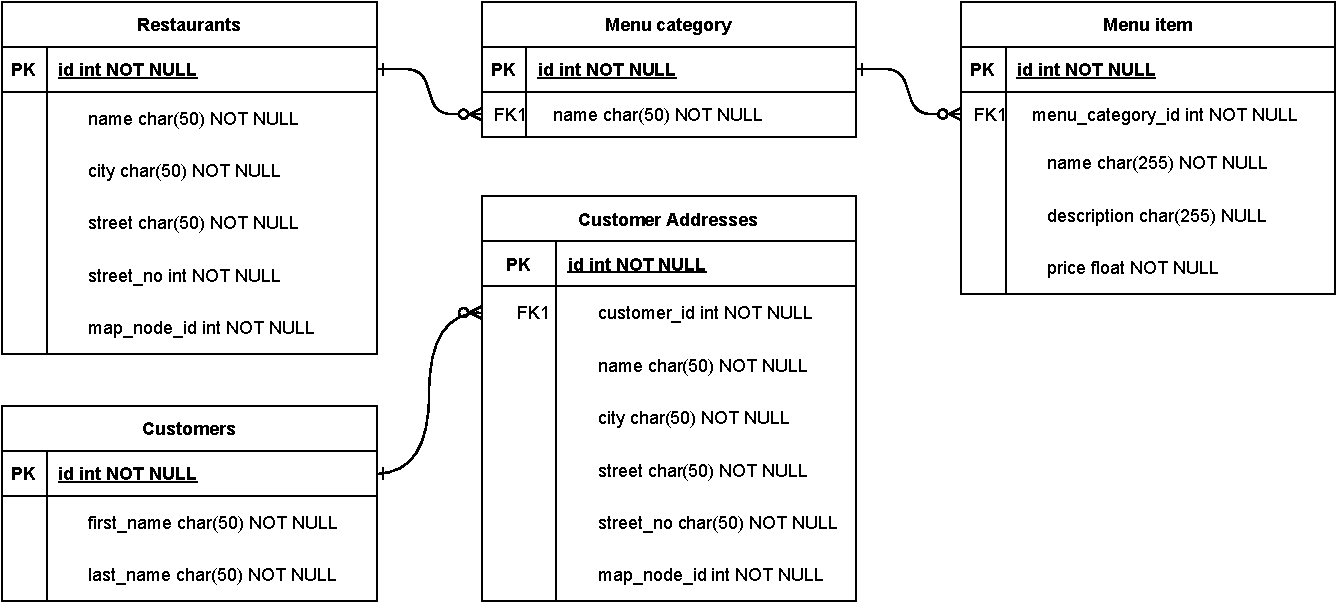
\includegraphics[width=0.9\linewidth]{img/er.drawio.pdf}
			\caption{Relational data model: entity relationship diagram}
			\label{fig:er}
		\end{figure}
	
	\subsection{Non-relational data}\label{sec:nonrelational-data}
		There are 2 parts to the non-relational data in this system: Map and Orders
		\paragraph{Orders} are saved in a document database and they usually have similar structure, which can be describe using the following schema bellow. Orders are the most commonly manipulated data in the entire system - they are used  for keeping track of the orders, order history, and delivery status and as such must be always available and very responsive. 
		
		\begin{lstlisting}[language=json]
{
	"$schema": "http://json-schema.org/draft-04/schema#",
	"title": "Food delivery order",
	"description": "This document records the details of a food delivery order",
	"type": "object",
	"properties": {
		"id": {
			"description": "A unique identifier for an order",
			"type": "number"
		},
		"created_at": {
			"description": "Unix timestamp of order creation",
			"type": "number"
		},
		"restaurant": {
			"description": "Restaurant this was ordered from",
			"type": "object",
			"properties": {
				"id": {},
				"name": {},
				"map_node_id": {
					"description": "Restaurant location map node ID",
					"type": "number"
				}
			}
		},
		"customer_id": {
			"description": "ID of the customer in the relational DB",
			"type": "number"
		},
		"menu_items": {
			"description": "Ordered menu items",
			"type": "array",
			"items": {
				"description": "Menu item",
				"type": "object",
				"properties" {
					"id": {
						"description": "ID of the menu item",
						"type": "number"
					},
					"name": {
						"description": "Name of the menu item",
						"type": "string"
					},
					"price": {
						"description": "Price of the menu item at the time of the order",
						"type": "number"
					},
				}
			}
		},
		"delivery": {
			"status": {
				"description": "Status of this order",
				"type": "string",
			},
			"courier_position": {
				"map_node_id": {
					"description": "ID of a map node in neo4j",
					"type": "number"
				}
			},
			"destination": {
				"description": "Object describing the delivery location",
				"type": "object",
				"properties": {
					"address": {
						"description": "Formatted address to be displayed in order detail",
						"type": "string"
					},
					"map_node_id": {
						"description": "ID of a map node in neo4j",
						"type": "number"
					}
				}
			}
		}
	}
}
		\end{lstlisting}
	
		\paragraph{Map} The map model is designed to be saved in a graph DB and closely copies the model of \href{https://wiki.openstreetmap.org/wiki/OSM_XML}{OpenStreetMap XML} in the sense, that all junctions are graph nodes and the connections between them are graph edges. The map is more or less stable, will only be altered sporadically, but the readability of these data is crucial for navigation and delivery, making it very important part of the system. The shortest path queries also shouldn't take too long, but a latency of few seconds is acceptable.
		

\section{System architecture}
	The application will be written in \href{https://rust-lang.org}{Rust} using the \href{https://github.com/seanmonstar/warp}{Warp framework}. The system will not have any frontend UI and will accept commands and queries using REST API.
	
	\subsection{DB systems}
		The chosen DB systems reflect the data types and needs describe in \ref{sec:data}. For relational data I've chosen to use the \href{https://www.cockroachlabs.com/product/}{CockroachDB} as it is a scalable SQL database with good support and PostgreSQL syntax resulting in very good interoperability.
		
		The map data will be stored in \href{https://neo4j.com/}{neo4j}, which is a graph DB allowing us to use some of the shortest path algorithms in its library and the Orders data will be stored in \href{https://www.mongodb.com/}{MongoDB} which is very fast, scalable document NoSQL DB.
	
	\subsection{Operations and CQRS}
		The system will use REST API and will implement CQRS using separate endpoints and handlers (either command or query) for every operation.
		
		Basic CRUD (create, read, update, delete) operations will be created for \texttt{Restaurants}, \texttt{Customers}, \texttt{Addresses}, \texttt{Menu categories}, \texttt{Menu items}, \texttt{Orders} entities. Furthermore there will be operations to calculate the best route for delivery, and find restaurants near customer. For each of these operations a new structure called either \texttt{<op>Command} or \texttt{<op>Query} will be created. This structure will then cover the whole operation execution resulting in a clear architecture.
		
		\begin{figure}[h]
			\centering
			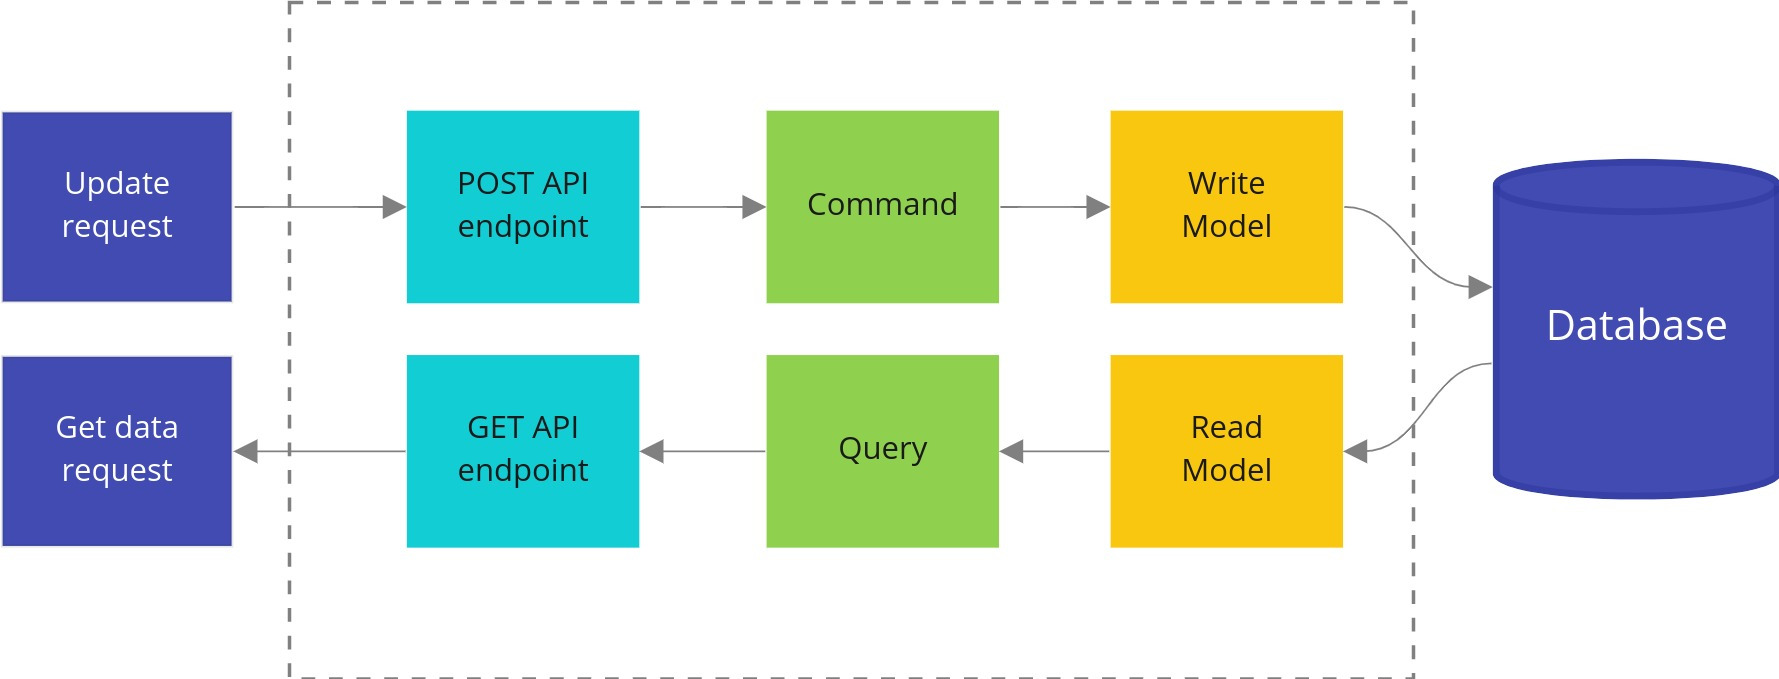
\includegraphics[width=0.7\linewidth]{img/cqrs-architecture}
			\caption{CQRS architecture {\tiny (\href{https://threedots.tech/post/basic-cqrs-in-go/}{source})}}
			\label{fig:cqrs-architecture}
		\end{figure}

	
%\newpage
%\nocite{*}
%\bibliography{references}
\end{document}